\documentclass[tikz,border=0pt]{standalone}
%% Shared style for the figures: TUHH colour palette, Latin Modern fonts.
%% Highlights are bold at caption size (10 pt); longer text is regular and
%% 2 pt smaller (8 pt). Figures are drawn at the text width of the
%% manuscript (390 pt) and must be included unscaled.
\usepackage[T1]{fontenc}
\usepackage{lmodern}
\usepackage{graphicx}
\usepackage{tikz}
\usetikzlibrary{arrows.meta,positioning,calc,fit,backgrounds}

\definecolor{tuhhturquoise}{HTML}{00C1D4}
\definecolor{tuhhyellow}{HTML}{FFDE36}
\definecolor{tuhhred}{HTML}{FF4F4F}
\definecolor{tuhhmint}{HTML}{5AFFC5}
\definecolor{tuhhcoolgray}{HTML}{D0D0CE}
\definecolor{tuhhpurple}{HTML}{7200FE}
\definecolor{tuhhwarmgray}{HTML}{A8968C}
\colorlet{ink}{black!85}

\newcommand{\hl}[1]{{\fontsize{10}{12}\selectfont\bfseries #1}}
\newcommand{\tx}[1]{{\fontsize{8}{9.6}\selectfont #1}}
\newcommand{\txi}[1]{{\fontsize{8}{9.6}\selectfont\itshape #1}}

%% \logo{file stem}{height}{fallback wordmark}: uses logos/<stem>.pdf or
%% .png when present, and a typeset wordmark otherwise.
\newcommand{\logo}[3]{%
  \IfFileExists{logos/#1.pdf}{\includegraphics[height=#2]{logos/#1.pdf}}{%
  \IfFileExists{logos/#1.png}{\includegraphics[height=#2]{logos/#1.png}}{%
  {\fontsize{10}{12}\selectfont\bfseries\sffamily #3}}}}

\tikzset{
  x=1pt, y=1pt, text=ink,
  card/.style={draw=tuhhcoolgray, line width=0.8pt, rounded corners=3pt,
               fill=white},
  band/.style={rounded corners=3pt, draw=none},
  flow/.style={-{Stealth[length=5pt,width=4.5pt]}, line width=1pt,
               draw=ink},
  gap/.style={draw=tuhhred, line width=1pt, dash pattern=on 3pt off 2pt},
  lbl/.style={inner sep=0pt, outer sep=0pt, align=left, anchor=north west},
  tag/.style={fill=tuhhyellow, rounded corners=2pt, inner xsep=3pt,
              inner ysep=1.5pt, anchor=west},
}

\begin{document}
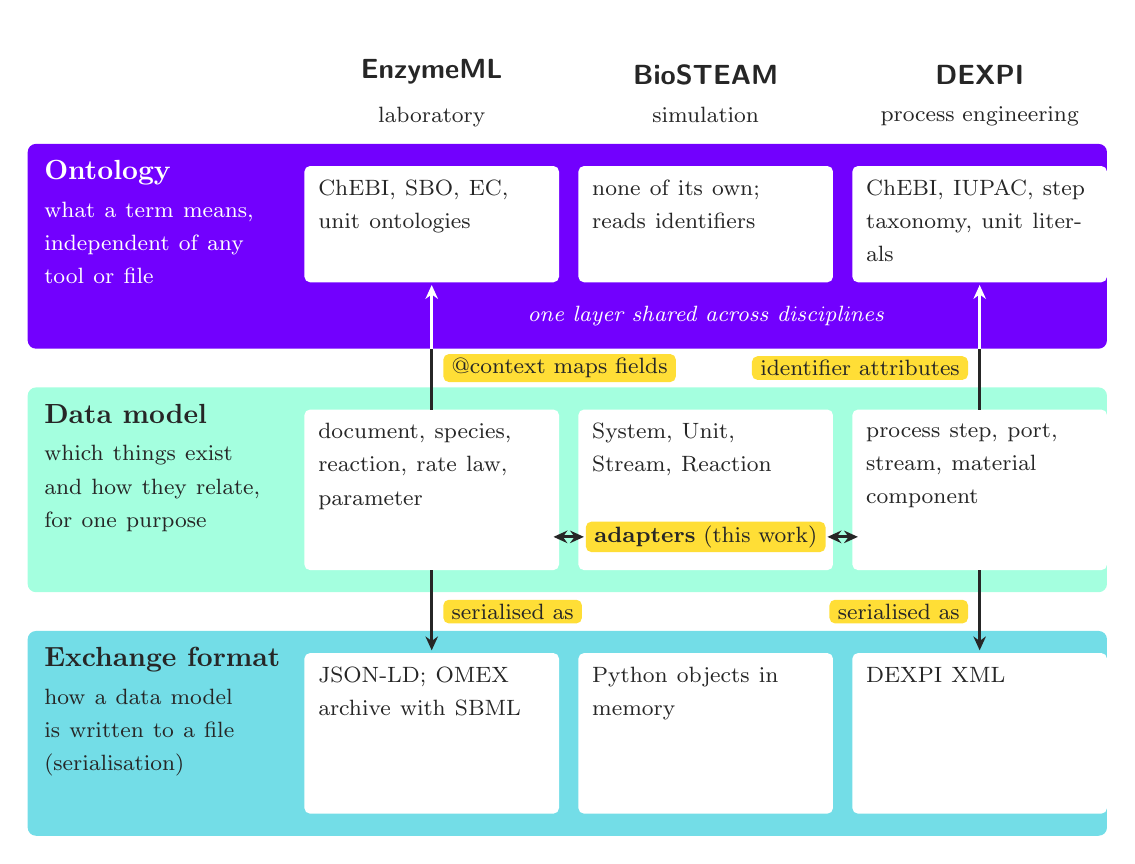
\begin{tikzpicture}
\useasboundingbox (0,0) rectangle (390,292);

% column headers (x: labels 0-92, columns 100-192, 199-291, 298-390)
\node[anchor=south] at (146,268) {\logo{enzymeml}{11pt}{EnzymeML}};
\node[anchor=south] at (245,268) {\logo{biosteam}{12pt}{BioSTEAM}};
\node[anchor=south] at (344,268) {\logo{dexpi}{11pt}{DEXPI}};
\node[anchor=north] at (146,267) {\tx{laboratory}};
\node[anchor=north] at (245,267) {\tx{simulation}};
\node[anchor=north] at (344,267) {\tx{process engineering}};

% --- ontology row (spans all disciplines) ---------------------------------
\fill[band, tuhhpurple] (0,176) rectangle (390,250);
\node[lbl, text=white] at (6,244) {\hl{Ontology}};
\node[lbl, text=white, text width=84pt] at (6,229)
  {\tx{what a term means, independent of any tool or file}};
\foreach \x/\t in {100/{ChEBI, SBO, EC, unit ontologies},
                   199/{none of its own; reads identifiers},
                   298/{ChEBI, IUPAC, step taxonomy, unit literals}}{
  \fill[white, rounded corners=2pt] (\x,200) rectangle (\x+92,242);
  \node[lbl, text width=82pt] at (\x+5,237) {\tx{\t}};
}
\node[anchor=center, text=white] at (245,188)
  {\txi{one layer shared across disciplines}};

% --- data model row --------------------------------------------------------
\fill[band, tuhhmint!55] (0,88) rectangle (390,162);
\node[lbl] at (6,156) {\hl{Data model}};
\node[lbl, text width=84pt] at (6,141)
  {\tx{which things exist and how they relate, for one purpose}};
\foreach \x/\t in {100/{document, species, reaction, rate law, parameter},
                   199/{System, Unit, Stream, Reaction},
                   298/{process step, port, stream, material component}}{
  \fill[white, rounded corners=2pt] (\x,96) rectangle (\x+92,154);
  \node[lbl, text width=82pt] at (\x+5,149) {\tx{\t}};
}

% --- serialisation row -----------------------------------------------------
\fill[band, tuhhturquoise!55] (0,0) rectangle (390,74);
\node[lbl] at (6,68) {\hl{Exchange format}};
\node[lbl, text width=84pt] at (6,53)
  {\tx{how a data model is written to a file (serialisation)}};
\foreach \x/\t in {100/{JSON-LD; OMEX archive with SBML},
                   199/{Python objects in memory},
                   298/{DEXPI XML}}{
  \fill[white, rounded corners=2pt] (\x,8) rectangle (\x+92,66);
  \node[lbl, text width=82pt] at (\x+5,61) {\tx{\t}};
}

% --- vertical relations ----------------------------------------------------
\foreach \x in {146,344}{
  \draw[flow] (\x,96) -- (\x,67);
  \draw[line width=1pt, draw=ink] (\x,154) -- (\x,176);
  \draw[flow, draw=white] (\x,176) -- (\x,199);
}
\node[tag] at (150,81) {\tx{serialised as}};
\node[tag, anchor=east] at (340,81) {\tx{serialised as}};
\node[tag] at (150,169) {\tx{@context maps fields}};
\node[tag, anchor=east] at (340,169) {\tx{identifier attributes}};

% --- adapters (this work) --------------------------------------------------
\draw[flow, {Stealth[length=5pt,width=4.5pt]}-{Stealth[length=5pt,width=4.5pt]}]
  (190,108) -- (201,108);
\draw[flow, {Stealth[length=5pt,width=4.5pt]}-{Stealth[length=5pt,width=4.5pt]}]
  (289,108) -- (300,108);
\node[tag, anchor=center] at (245,108) {\tx{\textbf{adapters} (this work)}};
\end{tikzpicture}
\end{document}
